
\chapter{Album 9}
\thispagestyle{empty} %本页頁碼空白
\vspace{-16mm}
\LARGE {時間(とき)の翼}

\normalsize{JBCJ-1033 2001.2.15 \ release}
\\

\vspace{-5mm}

\parpic[l]{
\pichskip{6em}
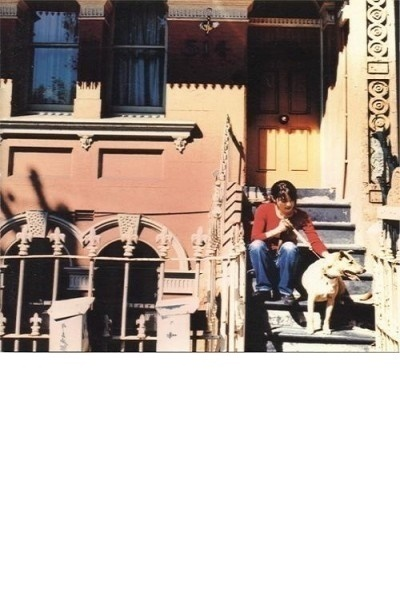
\includegraphics[width=0.4\textwidth]{9.jpg}}

\small{\hyperlink{9_0}{1.Get U're Dream}}

\tiny{作詞:坂井泉水 \ 作曲:大野愛果 \ 編曲:葉山たけし}

\small{\hyperlink{9_1}{2.この涙 星になれ}}

\tiny{作詞:坂井泉水 \ 作曲:岩井勇一郎 \ 編曲:古井弘人}

\small{\hyperlink{9_2}{3.promised you ~with P-edition~}}

\tiny{作詞:坂井泉水 \ 作曲:栗林誠一郎 \ 編曲:Cybersound}

\small{\hyperlink{9_3}{4.痛いくらい君があふれているよ}}

\tiny{作詞:坂井泉水 \ 作曲/編曲:シオジリケンジ}

\small{\hyperlink{9_4}{5.窓の外はモノクローム}}

\tiny{作詞:坂井泉水 \ 作曲:岩井勇一郎 \ 編曲:大賀好修}

\small{\hyperlink{9_5}{6.お・も・ひ・で}}

\tiny{作詞:坂井泉水 \ 作曲:寺尾広 \ 編曲:古井弘人}

\small{\hyperlink{9_6}{7.明日もし君が壊れても}}

\tiny{作詞:坂井泉水 \ 作曲:大野愛果 \ 編曲:徳永暁人}

\small{\hyperlink{9_7}{8.世界はきっと未来の中}}

\tiny{作詞:坂井泉水 \ 作曲:岩井勇一郎 \ 編曲:徳永暁人/古井弘人/シオジリケンジ}

\small{\hyperlink{9_8}{9.hero}}

\tiny{作詞:坂井泉水 \ 作曲:大野愛果 \ 編曲:大賀好修}
\begin{comment}
\small{\hyperlink{9_9}{10.揺れる想い Gomi's New York Remix}}

\small{\hyperlink{9_10}{11.負けないで Gomi's 10th Anni. Special Mix}}
\end{comment}

\small{\hyperlink{9_9}{10.時間の翼}}

\tiny{作詞:坂井泉水 \ 作曲:大野愛果 \ 編曲:徳永暁人}

\clearpage
